\section{Ethernet und LAN}
\subsubsection{Local Area Networks (LAN)}

    \centering
    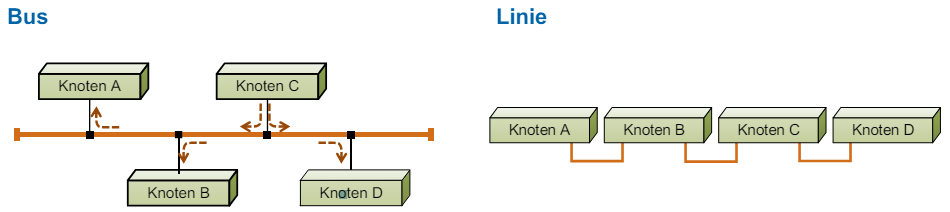
\includegraphics[width=0.9\linewidth]{images/bus_linie_topo.png}\\
    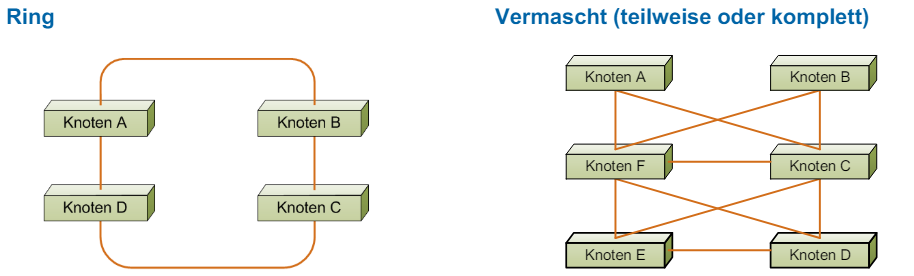
\includegraphics[width=0.9\linewidth]{images/ring_vermascht_topo.png}\\
    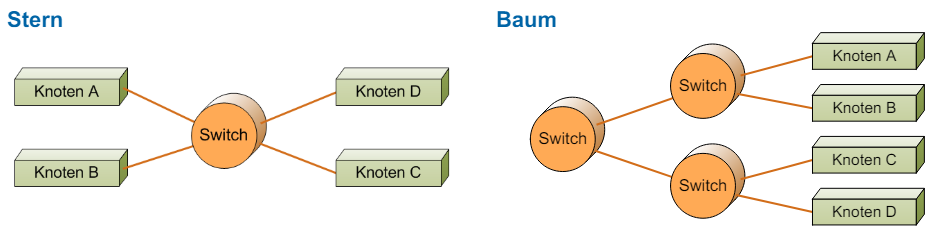
\includegraphics[width=0.9\linewidth]{images/stern_baum_topo.png}

\subsubsection{Übertragung und Adressierung}

\begin{definition}{Übertragungsarten}
    Immer genau 1 Sender, E = \# Empfänger
    
    \begin{minipage}{0.35\linewidth}
        \includegraphics[width=0.4\linewidth, angle=90]{images/übertragungsarten.png}
    \end{minipage}
    \begin{minipage}{0.6\linewidth}
        \begin{itemize}
            \item Unicast: 1 E 
            \item Multicast: n E (Gruppe)
            \item Broadcast: alle Knoten im LAN
        \end{itemize}
    \end{minipage}
\end{definition}


\begin{formula}{IEEE MAC Adressen}
    \begin{itemize}
        \item 3-Byte «OUI» identifiziert Hersteller
        \item 3-Byte Laufnummer durch Hersteller verwaltet
    \end{itemize}
    Klassifizierung der MAC Adresse:\\
    \begin{minipage}{0.6\linewidth}
    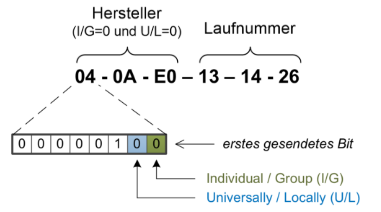
\includegraphics[width=1\linewidth]{images/klassifizierung_MAC_adresse.png}
    \end{minipage}
    \begin{minipage}{0.38\linewidth}
        Individual/Group Bit:
        \begin{itemize}
            \item 0 = individual address
            \item 1 = group address
        \end{itemize}
        Universally/Locally Bit:
        \begin{itemize}
            \item 0 = universally administrated adress
            \item 1 = locally administrated adress
        \end{itemize}
    \end{minipage}
\end{formula}

\begin{example2}{Ethernet Frame Format und MAC-Adresse}\\
    Sende Ethernet-Frame über 100BASE-TX Schnittstelle, Bit-Sequenz auf Kabel:\\
    10101010 10101010 10101010 10101010 10101010 10101010\\
    10101010 10101011 00010000 00000000 01011010 11100011\\
    10011111 10000110 ...\\
    MAC-Adresse und Hersteller des Empfängers:
    \begin{itemize}
        \item 7 Bytes Präambel (10101010), 1 Byte SFD (10101011)
        \item 6 Bytes Destination Address: 00001000 (=08) 00000000 (=00) 01011010 (=5A) 11000111 (=C7) 11111001(=F9) 01100001(=61)
    \end{itemize}
    $\Rightarrow$ MAC-Adresse: 08-00-5A-C7-F9-61, Hersteller (08-00-5A) IBM
\end{example2}

\begin{remark}
    Pro Byte zuerst LSB, dann MSB (Ausnahme Zahlenwerte, z.B. Length/Type-Feld)
\end{remark}

\subsubsection*{Ethernet}

\begin{definition}{Ethernet Frame Format}\\
    \begin{minipage}{0.3\linewidth}
        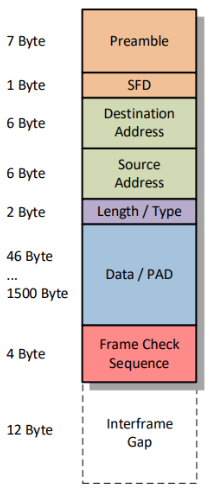
\includegraphics[width=0.9\linewidth]{images/ethernet_format.png}
    \end{minipage}
    \begin{minipage}{0.7\linewidth}
        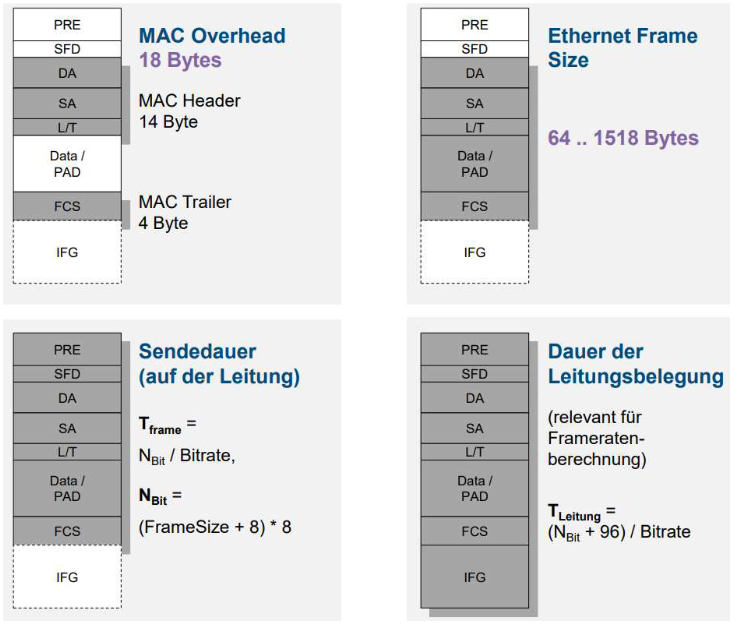
\includegraphics[width=1\linewidth]{images/ethernet_frame_details.png}
    \end{minipage}     
\end{definition}

\begin{theorem}{Bezeichnungsschema und Datenraten}\\
    \begin{minipage}{0.65\linewidth}
        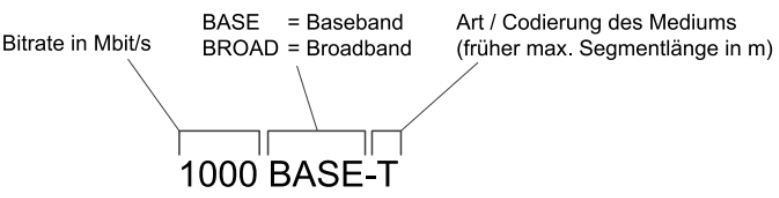
\includegraphics[width=1\linewidth]{images/ethernet_bezeichnungsschema.png}
    \end{minipage}
    \begin{minipage}{0.3\linewidth}
        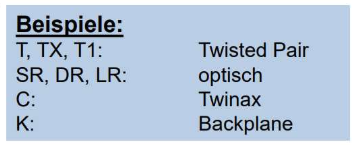
\includegraphics[width=1\linewidth]{images/ethernet_bsp_bezeichnung.png}
    \end{minipage}
\end{theorem}

\begin{concept}{Autonegation}
    Ermittlung der besten Betriebsart durch Austausch der Leistungsmerkmale zweier Netzwerkkomponenten\\
    Link Pulses:
    \begin{itemize}
        \item NLP = Link Presence Detection
        \item FLP = Autonegotiation, Autopolarity
    \end{itemize}
        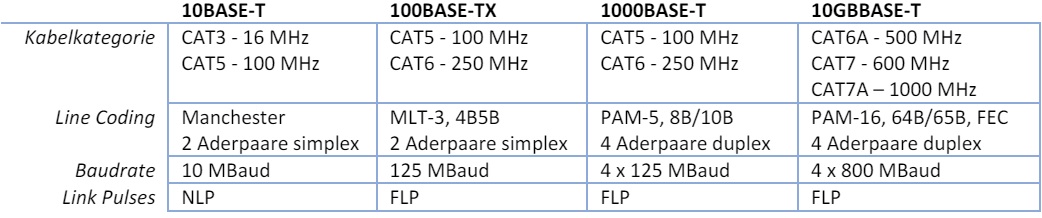
\includegraphics[width=1\linewidth]{images/ethernet_systeme.png}
\end{concept}


\paragraph{Ethernet Geräte (Network Gear)}

\begin{definition}{Switch/Brigde} Signale weiterleiten und verstärken, zusätzlich:
    \begin{itemize}
        \item Prüft Checksumme und kann Layer-2 Adressen auswerten
        \item Transparent: sollen für Endgeräte unsichtbar sein
        \item Verwendet Filtering Database (Adress-Learning)
    \end{itemize}
\end{definition}

\begin{theorem}{Merkmale von Switches und Bridges}\\
    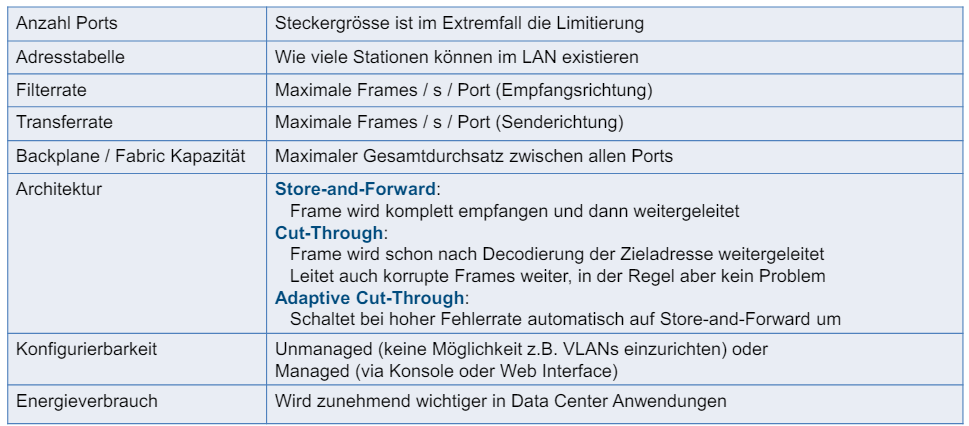
\includegraphics[width=1\linewidth]{images/merkmale_switches_bridges.png}
\end{theorem}


\begin{definition}{Filtering Database}
    Mapped MAC-Adressen auf Ports, lernt nur Absenderadresse \\
    Adresse bekannt $\rightarrow$ direkt, sonst Flooding (Broadcast/Multicast)\\
    \begin{centering}
        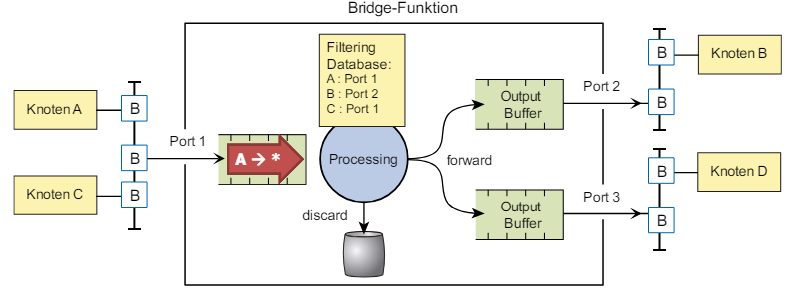
\includegraphics[width=0.9\linewidth]{images/filtering_database.png}    
    \end{centering}
\end{definition}

\begin{KR}{Weg/Zeit-Diagramm für das Senden eines Frames}\\
    \begin{minipage}{0.5\linewidth}
        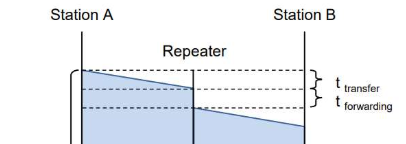
\includegraphics[width=1\linewidth]{images/zeit_frame_hub.png} 
        $$Latenz = t_{frame} + t_{transfer}$$
        $$t_{frame} = \frac{Framesize}{Bitrate}$$
        $$t_{transfer} = \frac{Distanz}{C_{Medium}}$$
        $t_{forwarding}$ \\kann verlängert werden um Verarbeitungszeit zu ermöglichen
    \end{minipage}
    \begin{minipage}{0.5\linewidth}
        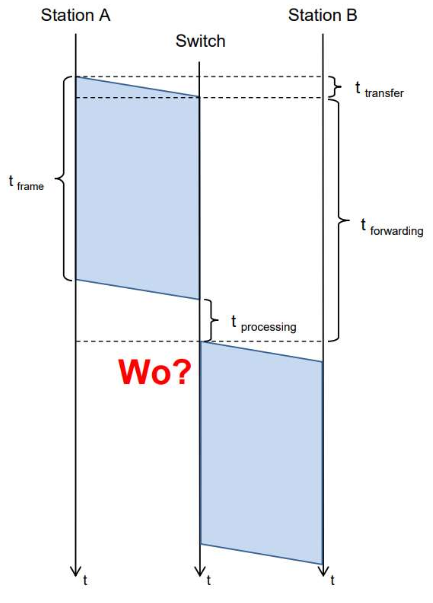
\includegraphics[width=1\linewidth]{images/weg_zeit_senden_frame.png}
    \end{minipage}
\end{KR}

\begin{formula}{Kollisionserkennung}
    können durch Überlagerung von Signalen entstehen. Kollisionen müssen erkannt werden!\\
        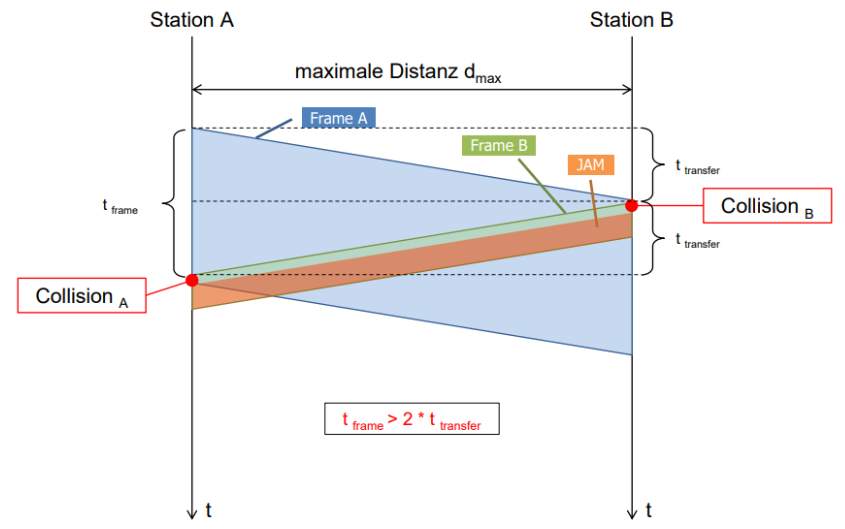
\includegraphics[width=0.9\linewidth]{images/kollisionserkennung_lan.png}\\
    Bedingungen für Kollisionserkennung:
    \begin{itemize}
        \item Ohne Repeater: $t_{frame} > 2 \cdot t_{transfer}$
        \item Mit Repeater: $t_{frame} > 2 \cdot (\sum t_{transfer} + \sum t_{forwarding})$
    \end{itemize}
    Ein Knoten kann Kollisionen nur lokal erkennen, solange er selbst am Senden ist
    $$d_{max} < \frac{1}{2} \cdot \frac{Framesize_{min}}{Bitrate} \cdot C_{Medium}, d_{max} < \frac{1}{2} \cdot \frac{576 Bit}{10 \cdot 10^6 \cdot Bit/s}$$
\end{formula}

\subsubsection{Redundanz (Spanning Tree)}

\begin{KR}{Spanning Tree Algorithmus}\\
    Ziel: Redundante Pfade $rightarrow$ Probleme! $\Rightarrow$ Alle Segmente loop-frei verbinden\\
    Initialisierung
    \begin{itemize}
        \item Alle Ports für Nutzdaten blockiert
        \item Annahme: «Ich bin Root»
        \item Austausch BPDUs mit Nachbarn (Root ID, Root Cost, Bridge ID, Port ID)
    \end{itemize}
    Aufbau des Spanning Tree
    \begin{itemize}
        \item «kleinster» Nachbar als Root gesetzt $\rightarrow$ Anzahl Hops + 1 (Beachte Prioritätswert)
        \item wiederholen bis alle dieselbe Root ID haben
    \end{itemize}
    Setzen der Port Roles
    \begin{itemize}
        \item Root-Ports (Empfang der «besten» BPDU)
        \item Designated-Ports (Gegenstück zu Root-Ports)
        \item Weg zum «kleinsten» Nachbar wird bevorzugt (ID, Anzahl Hops)
        \item Alle anderen Ports bleiben blockiert (Discarding)
    \end{itemize}
        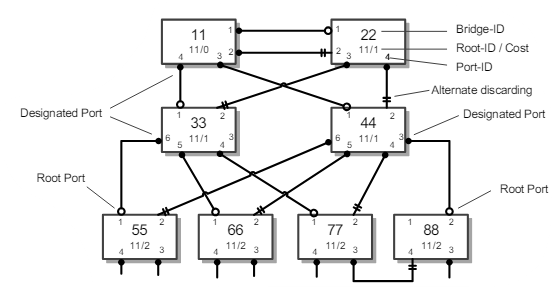
\includegraphics[width=0.8\linewidth]{images/spanning_tree_algorithmus.png}
\end{KR}

\begin{example}
    \begin{minipage}{0.48\linewidth}
        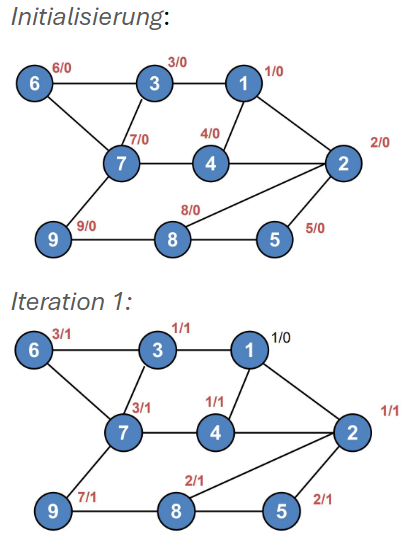
\includegraphics[width=1\linewidth]{images/rapid_spanning_tree1.png}
    \end{minipage}
    \begin{minipage}{0.48\linewidth}
        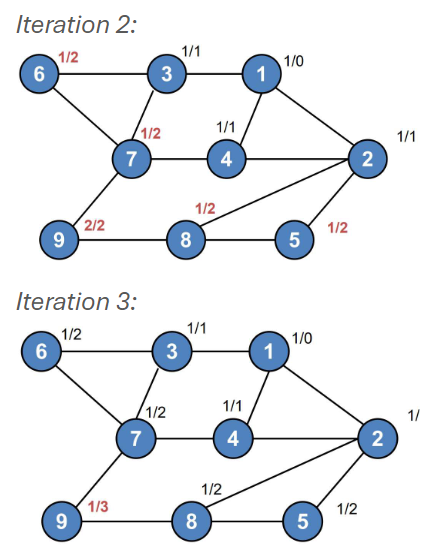
\includegraphics[width=1\linewidth]{images/rapid_spanning_tree2.png}
    \end{minipage}
    \begin{center}
    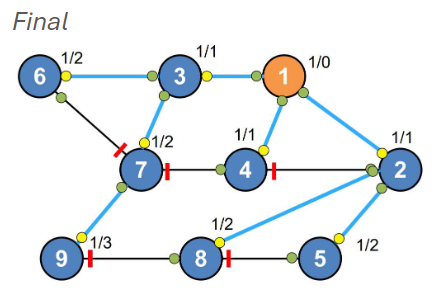
\includegraphics[width=0.55\linewidth]{images/rapid_spanning_tree3.png}
    \end{center}
\end{example}

\columnbreak

\subsection{Virtuelle LANs}

\begin{definition}{VLAN}
    Aufteilen eines LANs in mehrere unabhängige logische Netze (Broadcast Domains)\\
    \begin{minipage}{0.65\linewidth}
        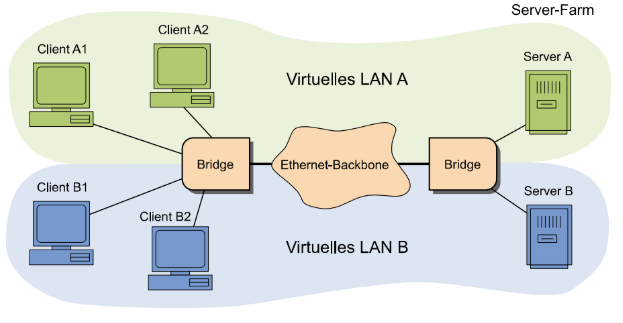
\includegraphics[width=1\linewidth]{images/vlan.png}
    \end{minipage}
    \begin{minipage}{0.3\linewidth}
        Trunk Links: \\
        Teil von mehreren VLANs $\rightarrow$ \\
        Frames eindeutig kennzeichnen!
        \vspace{1mm}\\
        Trunk = Tagged Access = Untagged
    \end{minipage}
\end{definition}

\begin{formula}{VLAN Tagging} \\
    \begin{minipage}{0.3\linewidth}
        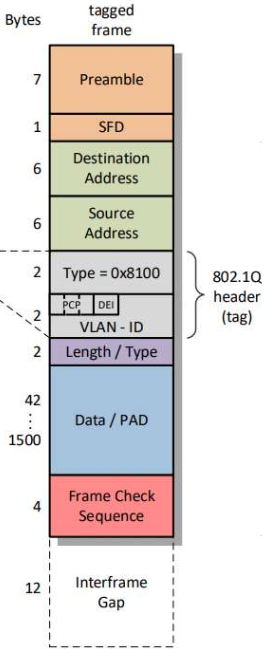
\includegraphics[width=1\linewidth]{images/vlan_tagging.png}
    \end{minipage}
    \begin{minipage}{0.65\linewidth}
        Erweiterung des Ethernet Headers durch einen VLAN-Tag (+ 4 Bytes)
        \vspace*{2mm}\\
        VLAN-ID (VID) im VLAN-Tag
        \begin{itemize}
            \item Zuordnung 
        \end{itemize}
        Priority Code Point (PCP)
        \begin{itemize}
            \item ermöglicht Priorisierung
        \end{itemize}
        Discard Eligibility Indicator (DEI) 
        \begin{itemize}
            \item 0 $\rightarrow$ Frame wird bei Überlastung zuerst verworfen
        \end{itemize}
        Vorteile: 
        \begin{itemize}
            \item Transparent für Endgeräte 
            \item VLAN Konfiguration nur im Netz (dh einfach)
        \end{itemize}
    \end{minipage}
\end{formula}



\begin{example}
    Gesendete Frames:
    \begin{center}
    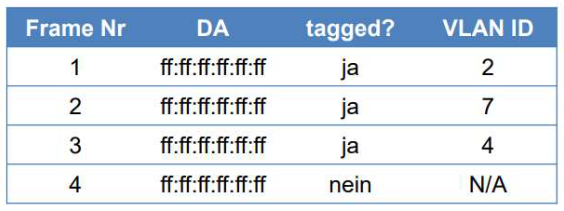
\includegraphics[width=0.5\linewidth]{images/bsp_vlan.png}
    \end{center}
    Switch Konfiguration:
    \begin{center}
    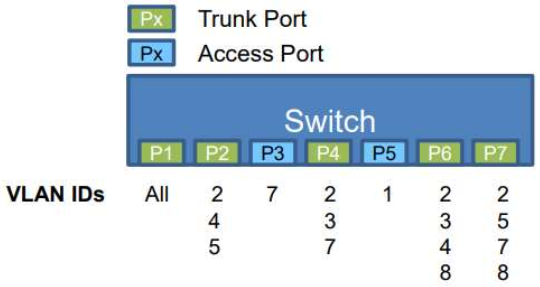
\includegraphics[width=0.5\linewidth]{images/vlan_example_switch.png}
    \end{center}
    Welche Frames werden an welchen Ports gesendet und sind diese getagged oder ungetagged?
    \begin{center}
    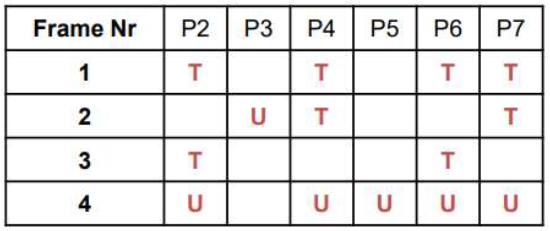
\includegraphics[width=0.5\linewidth]{images/vlan_example_frames.png}
    \end{center}
\end{example}

\begin{comment}
\begin{example}
    \begin{minipage}{0.38\linewidth}
        Switch Konfiguration:\\
        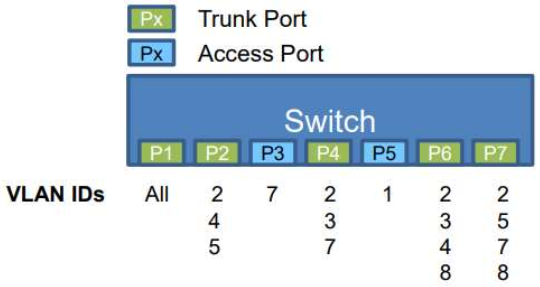
\includegraphics[width=1\linewidth]{images/vlan_example_switch.png}\\
        VLAN IDs
    \end{minipage}
    \begin{minipage}{0.6\linewidth}
        Gesendete Frames:\\
        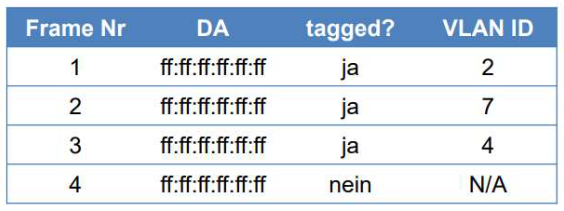
\includegraphics[width=1\linewidth]{images/bsp_vlan.png}
    \end{minipage}
    
    \begin{minipage}{0.5\linewidth}
        Welche Frames werden an welchen Ports gesendet und sind diese getagged oder ungetagged?
    \end{minipage}
    \begin{minipage}{0.5\linewidth}
        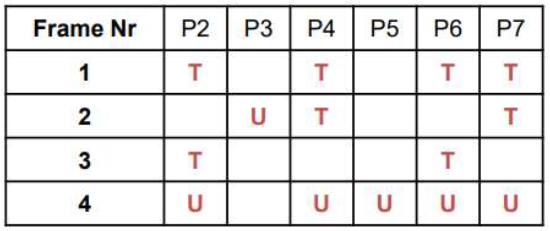
\includegraphics[width=1\linewidth]{images/vlan_example_frames.png}
    \end{minipage}    
\end{example}
\end{comment}







